\newpage
\maketitle
\begin{center}
\Large \textbf{第1章 行情数据处理} \quad 
\end{center}
\begin{abstract}
在本章中我们将通过AKshare库,获取A股分钟级行情数据,并将其进行预处理,变为深度学习可用的数据集。
\end{abstract}
\section{行情数据处理概述}
\subsection{获取原始行情数据}
我们首先通过apps.fmts.ds.akshare\_data\_source.AkshareDataSource获取原始的行情数据,-将其保存到csv文件中。如果存在该csv文件,则
直接从该文件中读出数据并返回。数据格式为:
\lstset{language=PYTHON, caption={行情数据格式}, label={c001-quotation-1-minute-bar}, basicstyle = \ttfamily}
\begin{lstlisting}
......
['2021-08-17 14:55:00', 30.339999999999996, 30.339999999999996, 30.339999999999996, 30.339999999999996, 200.0]
['2021-08-17 14:55:01', 30.339999999999996, 30.339999999999996, 30.339999999999996, 30.339999999999996, 200.0]
......
\end{lstlisting}
\subsection{行情数据预处理}
我们以收盘价为例,收盘价的折线图绘制程序如下所示:
\lstset{language=PYTHON, caption={收盘价折线图}, label={c001-close-price-curve-001}, basicstyle = \ttfamily}
\begin{lstlisting}
    class OhlcvProcessor(object):
    # 价格折线图模式
    PCM_DATETIME = 1
    PCM_TICK = 2

    @staticmethod
    def draw_close_price_curve(stock_symbol: str, mode=1) -> None:
        '''
        绘制收盘价折线图,横轴为时间,纵轴为收盘价
        '''
        data = AkshareDataSource.get_minute_bars(stock_symbol=stock_symbol)
        x = [v[0] for v in data[0:1000]]
        y = [v[4] for v in data[0:1000]]
        if mode == OhlcvProcessor.PCM_DATETIME:
            OhlcvProcessor._draw_date_price_curve(x, y)
        else:
            OhlcvProcessor._draw_tick_price_curve(y)

    def _draw_date_price_curve(x: List, y: List) -> None:
        x = [datetime.datetime.strptime(di, '%Y-%m-%d %H:%M:%S') for di in x]
        fig, axes = plt.subplots(1, 1, figsize=(8, 4))
        plt.rcParams['font.sans-serif']=['SimHei'] #用来正常显示中文标签
        plt.rcParams['axes.unicode_minus'] = False #用来正常显示负号
        # 最大化绘图窗口
        figmanager = plt.get_current_fig_manager()
        figmanager.window.state('zoomed')    #最大化
        # 绘制收盘价格折线图
        axes.plot_date(x, np.array(y), '-', label='Net Worth')
        # 设置横轴时间显示格式
        axes.xaxis.set_major_formatter(DateFormatter('%Y-%m-%d %H:%M:%S'))
        plt.gcf().autofmt_xdate()
        # 显示图像
        plt.show()
    
    def _draw_tick_price_curve(y: List) -> None:
        x = range(len(y))
        fig, axes = plt.subplots(1, 1, figsize=(8, 4))
        plt.rcParams['font.sans-serif']=['SimHei'] #用来正常显示中文标签
        plt.rcParams['axes.unicode_minus'] = False #用来正常显示负号
        # 最大化绘图窗口
        figmanager = plt.get_current_fig_manager()
        figmanager.window.state('zoomed')    #最大化
        # 绘制收盘价格折线图
        plt.title('收盘价折线图')
        axes.set_xlabel('时间刻度')
        axes.set_ylabel('收盘价')
        axes.plot(x, np.array(y), '-', label='Net Worth')
        plt.show()
\end{lstlisting}
代码解读如下所示:
\begin{itemize}
    \item 第3、4行:定义收盘价曲线绘制方式,一种是横轴为时间,另一种横轴为行情序号;
    \item 第6$\sim$10行:定义收盘价绘制方法,参数为股票代码和绘制模式,缺省值为横轴为时间(以分钟为单位),这种模式的缺点是从上一日收盘到下一日开盘有
    较大的时间间隔;
    \item 第11行:获取分钟线行情数据,格式为:[[dateteime, open, high, low, close, volume]];
    \item 第19行:以横轴为行情时间值绘制收盘价曲线;
    \begin{itemize}
        \item 第20行:将时间变为'2021-08-21 12:56:00'格式的列表;
        \item 第21行:设置显示图形;
        \item 第22行:设置字体使matplotlib可以正确显示汉字;
        \item 第23行:使matplotlib可以显示负号;
        \item 第24$\sim$26行:使matplotlib绘图窗口最大化;
        \item 第27、28行:绘制收盘价时间曲线;
        \item 第29$\sim$31行:设置横坐标轴时间显示格式为'2021-08-21 12:56:00',并自动调整为45度角倾斜,以节省显示空间;
    \end{itemize}
\end{itemize}
\begin{figure}[H]
	\caption{以时间为横轴的收盘价折线图}
	\label{f000001}
	\centering
	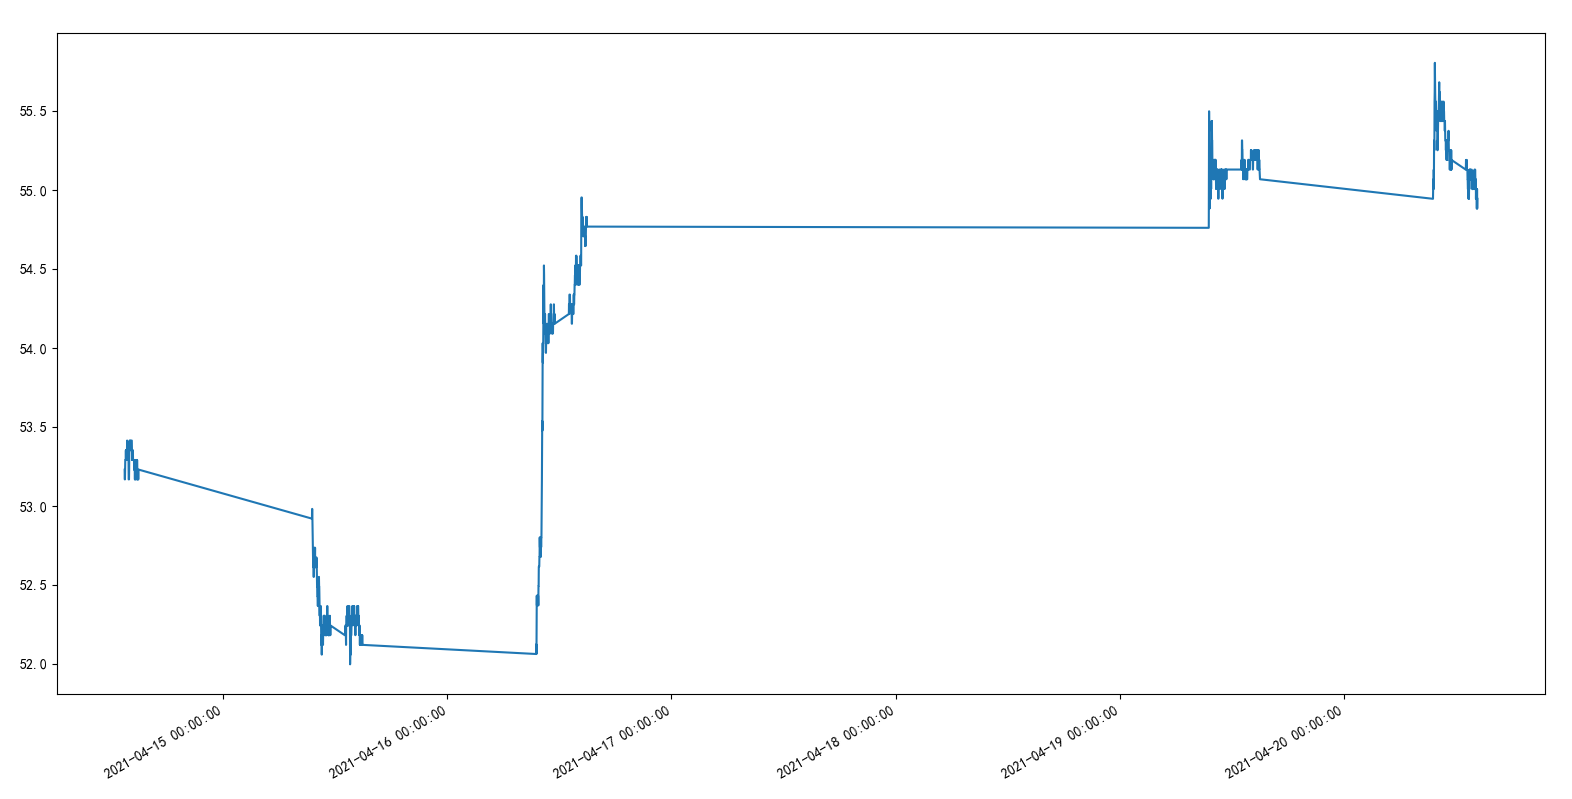
\includegraphics[width=10cm]{images/f000001}
\end{figure}
\begin{figure}[H]
	\caption{以序号为横轴的收盘价折线图}
	\label{f000002}
	\centering
	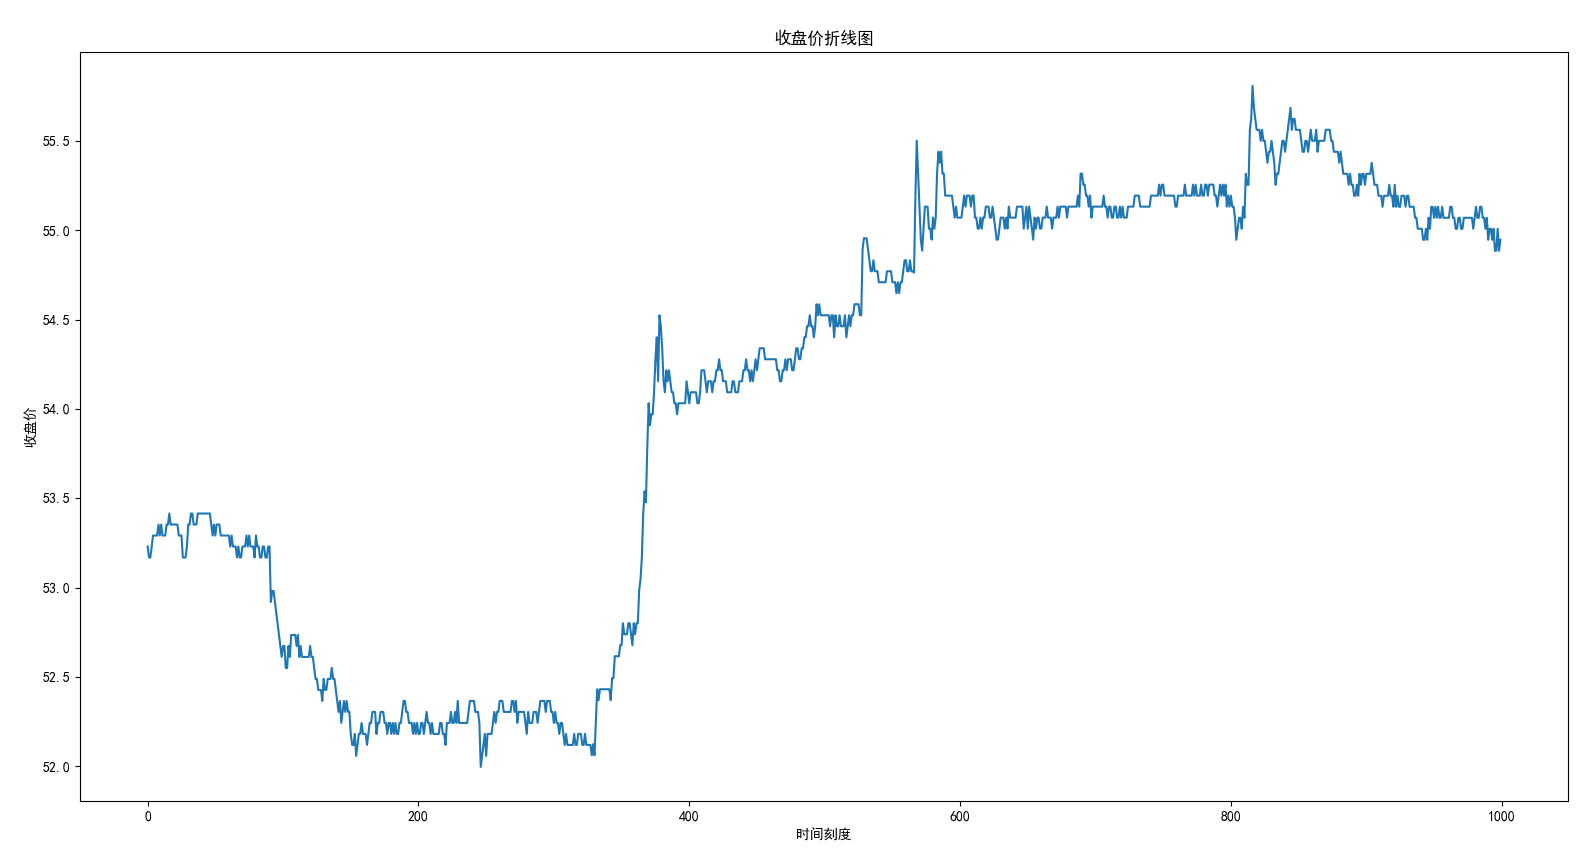
\includegraphics[width=10cm]{images/f000002}
\end{figure}
如\ref{f000001}所示,图中每天收盘到第二天开盘间没有行情数据,所以图形不太好看出规律,而图\ref{f000002}则可以较好的反映价格的变化规律,因此
我们在通常情况下,选择图\ref{f000002}的形式。





\section{最后}